\documentclass{article}
\usepackage{hyperref}
\usepackage{vmargin}
\usepackage{amsmath}
\usepackage{graphicx}
\setpapersize{USletter}
\setmarginsrb{1in}{1in}{1in}{1in}{0.25in}{0.25in}{0in}{0in}

\newcommand{\comment}[2]{[{\Large\sc #1:} \textsf{#2}]}

\newcommand{\doug}[1]{\comment{Doug}{#1}}
\newcommand{\gary}[1]{\comment{Gary}{#1}}
\newcommand{\jaakko}[1]{\comment{Jaakko}{#1}}

\begin{document}

\markboth{Doc. no: NXXXX=04-0XXX}{Doc. no: NXXXX=04-0XXX}
\pagestyle{myheadings}

\title{Variadic Templates}
\author{Douglas Gregor \and Jaakko J\"arvi \and Gary Powell}
\date{}
\maketitle

\par\noindent Document number: NXXXX=04-XXXX
\par\noindent Date: \today
\par\noindent Project: Programming Language C++, Evolution Working Group
\par\noindent Reply-to: Douglas Gregor $<${\tt gregod@cs.rpi.edu}$>$

\section{Introduction}
This proposal directly addresses two problems:
\begin{itemize}
\item The inability to instantiate class and function templates with an arbitrarily-long list of template parameters.
\item The inability to pass an arbitrary number of arguments to a function in a type-safe manner.
\end{itemize}

The proposed resolution is to introduce a syntax and semantics for
variable-length template argument lists (usable with function templates
via explicit template argument specification and with class templates)
along with a method of argument ``bundling'' using the same mechanism to
pass an arbitrary number of function call arguments to a function in a
typesafe manner.

\section{Motivation}
\subsection{Variable-length template parameter lists}
Variable-length template parameter lists (variadic templates) allow a
class or function template to accept some number (possibly zero) of
template arguments beyond the number of template parameters specified.
This behavior can be simulated in C++ via a long list of defaulted
template parameters, e.g., a typelist wrapper may appear as:

\begin{verbatim}
struct unused;
template<typename T1 = unused, typename T2 = unused, 
         typename T3 = unused, typename T4 = unused, 
         /* up to */ typename TN = unused> class list;
\end{verbatim}

This technique is used by various C++ libraries~\cite{Tuples01,
Jarvi02, Gurtovoy02}. Unfortunately, it leads to very
long type names in error messages (compilers tend to print the
defaulted arguments) and very long mangled names. It is also not
scalable to additional arguments without resorting to preprocessor
magic~\cite{Preprocessor01}. In all of these libraries (and presumably
many more), an implementation based on variadic templates would be
shorter and would not suffer the limitations of the aforementioned
implementation. The declaration of the {\tt list<>} template above may
be:
\begin{verbatim}
template<...> class list;
\end{verbatim}

\subsection{Typesafe Variable-length Function Parameter Lists}
Variable-length function parameter lists allow more arguments to be
passed to a function than are declared by the function. This feature
is rarely used in C++ code (except for compatibility with C
libraries), because passing non-POD types through an ellipsis ({\tt
  ...}) invokes undefined behavior. However, a typesafe form of such a
feature would be useful in many contexts, e.g., for implementing a
typesafe C++ {\tt printf} that works for non-POD types.

\section{Feature menu}
Prior versions of this proposal~\cite{GJP03,GJP04a} described various
points in the design space of variadic templates. In this version of
the proposal, we have chosen to enumerate the various potential design
decisions (mainly features) and discuss the impact of each on users
and compilers. Fig.~\ref{fig:dependencies} illustrates the
dependencies between features, such that an edge $A \rightarrow B$
indicates that feature $A$ requires acceptence of feature $B$, e.g.,
``Arbitrary matching patterns'' subsumes (and therefore requires
acceptence of) ``const/volatile/reference patterns''. 

\begin{figure}
\center
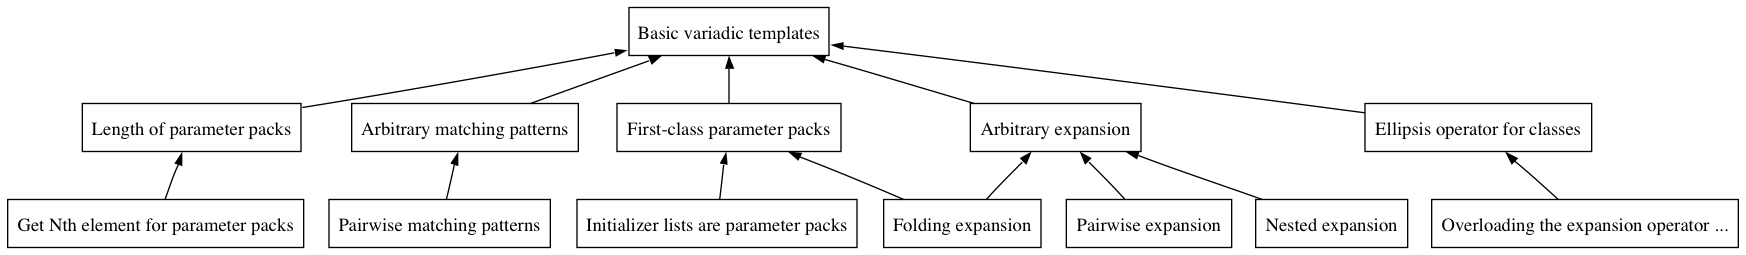
\includegraphics[width=6in,height=3in]{vt_deps}
\caption{Feature dependency graph for variadic templates}
\label{fig:dependencies}
\end{figure}

The following sections describe each feature listed in
Fig.~\ref{fig:dependencies}. Sec.~\ref{sec:menu} then provides several
``specials'': prepacked sets of features that work well together and
represent some overall goal for variadic templates. It is our hope
that the committee will select a special or a set of features
\textit{a la carte} for which we can draft a more formal
specification. 

\subsection{Basic variadic templates}
\label{sec:basic}
The most basic form of variadic templates requires the ability to
declare class/struct/union and function templates that accept an
arbitrary number of template arguments, declare function templates
that accept an arbitrary number of (function) arguments, and access
the ``extra'' template and function arguments.

We adopt the use of the ellipsis operator ``\texttt{...}'' to
represent variable-length argument lists. For variadic class templates
we allow ``\texttt{...}'' as the ``kind'' of the last template
parameter, which may optionally be followed by an identifier. The
following class template accepts one type argument followed by zero or
more other template arguments.

\begin{verbatim}
template<typename T, ... Tail> class tuple;

typedef tuple<int, float, double, std::string, 5, std::vector> t;
\end{verbatim}

Variadic function templates are declared similarly, allowing one to
explicitly specify any number of arguments:
\begin{verbatim}
template<... Args> void print_template_args();

print_template_args<int, 17, 42.0, &X::m>();
\end{verbatim}

We refer to \texttt{Tail} and \texttt{Args} as ``template parameter
packs'', because they pack together a set of template arguments into a
single parameter. In their most basic form, template parameter packs
provide only a single operation: unpacking via the ellipsis
(\texttt{...}) operator). Unpacking splits a template parameter pack
into its individual arguments, allowing each to be considered
individually. For instance, the following code builds a recursive
tuple from the types given:
\begin{verbatim}
template<typename Head, ... Tail> struct tuple { // #1
  Head head;
  tuple<Tail...> tail;
};

template<typename Head> struct tuple<Head> { // #2
  Head head;
};
\end{verbatim}

The instantiation of \texttt{tuple<int, double, std::string} uses the
primary template (\#1) with \texttt{Head}=\texttt{int} and
\texttt{Tail} containing \texttt{double} and \texttt{std::string},
which we denote by \texttt{Tail}=\texttt{<double, std::string>}. The
\texttt{tail} member is a tuple that will receive the template arguments
\texttt{double} and \texttt{std::string}, in that order, due to the
application of the \texttt{...} operator to the template parameter
pack \texttt{Tail}. 

The ellipsis operator represents both unpacking and packing arguments,
depending on context. For instance, a partial specialization can fix
some number of arguments and collect the rest in a template parameter
pack:

\begin{verbatim}
// Searching for two adjacenct types...
template<typename T, ... Elements> 
struct adjacent_find : adjacent_find<Elements...> { };

// Found adjacenct types!
template<typename T, ... Rest>
struct adjacent_find<T, T, Rest...> {
  static const bool value = true; 
  typedef T type;
};

// List is empty. We found nothing.
template<> struct adjacent_find { static const bool value = false; };
\end{verbatim}

Here, the partial specialization matches the case where two adjacent
types are the same and then collects the rest of the arguments into
the template parameter pack \texttt{Rest}. The ellipsis operator can
be applied to a parameter pack wherever there is a list of parameters
(for packing) or arguments (for unpacking), including:
\begin{itemize}
  \item In a partial specialization (e.g., the \texttt{adjacent\_find} example)
  \item In a \textit{template-id} (e.g., \texttt{tuple<Elements...>})
  \item In a function type (e.g., \texttt{void(int, ArgTypes...)})
\end{itemize}

The ellipsis operator also applies to \textit{value} parameter packs,
which store run-time values for type-safe variadic function
templates. For instance, a type-safe \texttt{printf} might be declared
as:

\begin{verbatim}
template<... Args> void printf(const char* s, Args args...);
\end{verbatim}

This declaration indicates that \texttt{printf} accepts a variable
number of parameters (both template and function arguments): the
\texttt{Args} template parameter pack contains the types of the
arguments, whereas the \texttt{args} template parameter pack contains
the values. The ellipsis operator following ``\texttt{args}''
indicates that extra arguments to \texttt{printf} should be bundled
into the \texttt{args} parameter pack and their types deduced and
placed into the \texttt{Args} template parameter pack.

The most basic formulation of variadic templates therefore consists
of:
\begin{itemize}
\item The ability to declare template and value parameter packs
\item The ability to unpack and pack template and value parameter
  packs via the ellipsis operator.
\item Partial ordering rules for class template partial
  specializations and function templates in the presence of variadic
  templates (discussed in a previous proposal~\cite{GJP04a}).
\end{itemize}

\subsection{First-class parameter packs}
\label{sec:first-class-pp}
In the basic formulation, template and value parameter packs are
merely bundles of parameters that have no direct representation within
the type system. However, we could make template parameter packs into
actual types---albeit special ones that permit the use of the ellipsis
operator---so that they could be passed to template arguments or
compared against each other. Moreover, value parameter packs now have
actual types based on the type of the associated template parameter
pack, and may become first-class objects templates. Thus they can be
default-constructed (if all types in them are default-constructible),
copy-constructed or assigned (if all types of copy-constructible or
assignable, respecitvely), and unpacked as needed. 

First-class parameter packs have some advantages over the basic
formulation of parameter packs, because it allows multiple arguments
to be stored together without resorting to recursion as with the
\texttt{tuple} template in Sec.~\ref{sec:basic}:
\begin{verbatim}
template<... Elements> 
class tuple
{
public:
  tuple(Elements elements...) : elements(elements) { }

private:
  Elements elements;
};
\end{verbatim}

Here we store members of every type in \texttt{Elements} in a single
parameter pack within the tuple, instead of creating a chain of
\texttt{tuple} instantiations where each stores a single element plus
the next \texttt{tuple} in the chain. 

\paragraph{User impact}: First-class parameter packs make writing some
heterogenous data structures simpler because they can eliminate the
need for recursive data structures. Performance (both compiler and
generated code) will improve because the number of instantiations
required to implement a heterogeneous data structure will be reduced
from ${\cal O}(N)$ to ${\cal O}(1)$. This effect has already been seen
when comparing the Boost.Tuples library~\cite{Tuples01}, which uses a
recursive data structure, to a preprocessor-based library, which
enumerates all data members. 

First-class parameter packs may be somewhat confusing to users,
because the distinction between a ``packed'' parameter pack and an
unpacked one becomes very important. For instance, if one forgets to
apply the ellipsis operator the compiler will pass the parameter pack
itself, e.g.,
\begin{verbatim}
template<... Args> void debugout(const std::string& s, Args args...)
{
  printf(("Debug: " + s).c_str(), args); // oops, should be "args..."
}
\end{verbatim}

\paragraph{Compiler impact}: First-class parameter packs introduce
more complexity into the implementation of variadic templates, because
the compiler must construct actual types and objects for each
parameter pack. In addition, there are some interesting interactions
between the object model used for parameter packs and the method by
which arguments are passed to function objects that require further
consideration; see~\cite{GJP04a}. 

\paragraph{Evaluation}: The most important realization with
first-class parameter packs is that they can be emulated via recursive
data structures. However, this emulation places an extra burden on
users and compilers, and is known to result in poorer performance.

\section{Initializer lists are parameter packs}
Initializer lists are typeless entities stored in the compiler that
can only be used in very restrictive ways for initializing
aggregates. We could lift some of the restrictions on initializer
lists by making them (value) parameter packs. This would permit writing
constructors and assignment operators that accept initializer lists,
e.g.,

\begin{verbatim}
template<... Elements>
class tuple
{
public:
  // #1: Build from an initializer list
  tuple(Elements elements) : elements(elements) { }

  // #2: Build from an initializer list, converting as necessary
  template<... Args> tuple(Args args) : elements(args...) { }

private:
  Elements elements;
};

// Passes initializer list as parameter pack to constructor #1
tuple<int, double, float> t1 = { 17, 3.14159, 2.718f };
  
// Passes initializer list as parameter pack to constructor #2
tuple<int, double, std::string> t2 = { 17, 3.14f, "foo" };
\end{verbatim}

Additionally, this change permits emulation of sequence
constructors~\cite{DoReStr03} via parameter packs, e.g.,
\begin{verbatim}
template<typename T>
class vector
{
public:
  template<... Elements> vector(Elements elements)
  {
    tr1::array<T, (pp_length<Elements>::value)> a = elements;
    assign(a.begin(), a.end());
  }
};
\end{verbatim}

The construction of \texttt{a} actually performs aggregate
initialization from the incoming parameter pack, which unfortunately
requires one extra copy. This copy can be elided by implementing the
constructor as a metaprogram\footnote{See Sec.~\ref{sec:pp-size} for a
  discussion of \texttt{pp\_length}}:

\begin{verbatim}
template<typename T>
class vector
{
public:
  template<... Elements> vector(Elements elements)
  {
    reserve(pp_length<Elements...>::value);
    do_push_back(elements...);
  }

  void push_back(const T&);

private:
  template<... Rest>
  void do_push_back(const T& x, Rest... rest) {
    push_back(x);
    do_push_back(rest...);
  }

  void do_push_back() {}
};
\end{verbatim}

\subsection{Ellipsis operator for classes}
One extension of the ellipsis operator would permit it to be applied
for any class type, which would have the effect of unpacking all of
the fields in that class type into separate arguments. This
information could be used for compile-time reflective metaprogramming,
e.g., to perform automatic marshalling or to construct property
inspectors. TBD TBD HERE HERE


\subsection{Length of parameter packs}
\label{sec:pp-size}
One can determine the number of elements in a template parameter pack
with the following template:
\begin{verbatim}
template<...> struct pp_length;

template<typename T, ... Rest>
struct pp_length<T, Rest...> {
  static const int value = 1 + pp_length<Rest...>::value; 
};

template<> struct pp_length<> {
  static const int value = 0;
};
\end{verbatim}

However, this requires ${\cal O}(N)$ instantiations for a parameter
pack of length $N$, which can be inefficient to compile. This option
proposed that unpacking a template or value parameter pack in a
\texttt{sizeof} expression will return its length, e.g.,

\begin{verbatim}
template<... Args>
  void f(Args... args)
  {
    const int num_args = sizeof(args...);
    // equivalent to...
    const int num_args = sizeof(Args...);
  }
\end{verbatim}

\subsection{Get Nth element for parameter pack}
Parameter packs are only accessible linearly, by peeling off arguments
at the front of the parameter pack. A general tuple, however, requires
the ability to access the $N^{\text{th}}$ element. For parameter
packs, we would like to be able to access the Nth element. For this we
propose to use the \texttt{[]} operator, but restrict the argument to
integral constant expressions because the result type differs
depending on the value of the argument. For instance,

\begin{verbatim}
template<... Args>
  void f(Args... args)
  {
    // Make copy of 2nd argument
    auto second = args[1];
  }
\end{verbatim}

We rely on \texttt{auto}~\cite{JarviStroustrup04} to deduce the type
of the argument for us. See Sec.~\ref{sec:nth-element-template} for an
alternative that introduces more syntax to enable access to the types
in a template parameter pack.

\subsection{Get Nth element for template parameter packs}
\label{sec:nth-element-template}
Given the \texttt{decltype}~\cite{JarviStroustrup04} extension, one
can build a metafunction that extracts the $N^{\text{th}}$ type in a
template parameter pack using ${\cal O}(1)$ instantiations:

\begin{verbatim}
template<... Args, std::size_t N>
  struct nth_type
  {
    static Args args;
    typedef decltype(args[N]) type;
  };
\end{verbatim}

Without \texttt{decltype}, we end up with an ${\cal
O}(N)$-instantiation metafunction.

\begin{verbatim}
template<std::size_t N, ...> struct nth_type_impl;

template<std::size_t N, typename T, ... Rest>
  struct nth_type_impl<N, T, Rest...>
    : nth_type_impl<N-1, Rest...> { };

template<typename T, ... Rest>
  struct nth_type_impl<0, T, Rest...>
  {
    typedef T type;
  };
  
template<... Args, std::size_t N>
  struct nth_type : nth_type_impl<N, Args...> { };
\end{verbatim}

This option involves introducing additional syntax for accessing the
$N^{\text{th}}$ type of a template parameter pack, using the new
\texttt{::[]} operator, e.g.,

\begin{verbatim}
template<... Args, typename R>
  struct function_traits<R (*)(Args...)>
  {
    typedef typename Args::[0] first_argument_type;
    typedef typename Args::[1] second_argument_type;
  };
\end{verbatim}

\textbf{Evaluation}: We sincerely hope that \texttt{decltype} will be
available in C++0x to make the \texttt{::[]} operator unnecessary. In
that case, permitting the \texttt{[]} operator on value parameter
packs is sufficient to provide this capability.

\subsection{Pairwise expansion}
Use zipping tuples as the example

\section{Syntax and Semantics}
\subsection{Variadic templates}
\par The template parameter list to a function or class template can
be declared to accept an arbitrary number of extra template arguments
by terminating it with ``...'' optionally followed by an identifier
through which these extra arguments can be accessed.
Any number of template
parameters may precede the ``...''. Thus we can define, for instance,
a class {\tt Foo} accepting a template type parameter followed by an
arbitrary number of template arguments as:
\begin{verbatim}
template<typename T, ... Args> class Foo;
\end{verbatim}

\noindent
Here, {\tt T} is the name of the template type parameter and {\tt
  Args} is the name of a ``template parameter pack'' containing the
(possibly empty) set of template arguments given to {\tt Foo}.
Template parameter packs may contain template type, non-type, and
template template arguments and are represented as an unspecified
class type when a type is required.

Function templates may also be variadic templates in the same manner
as class templates.  Arguments can be specified explicitly when
calling the function template, e.g:

\begin{verbatim}
template<... Args> void f();
// ... 
f<int, double>(); // Args will be contain <int, double>
\end{verbatim}
The next section describes when the types of the elements in 
a value parameter pack can be deduced from the argument types
of the call. 

\subsection{Typesafe variadic functions}
When a function template header contains a template parameter pack,
that template parameter pack may be used in the ``type'' of the final
function parameter, allowing the function to accept a variable number
of function parameters in a ``value parameter pack'' (or just
``parameter pack''). For instance, a typesafe C++ {\tt printf} may
be declared as:
\begin{verbatim}
template<... Args>
  void printf(const char* format, const Args&... args);
\end{verbatim}

\noindent The ellipsis indicates that the function ``parameter''
\texttt{args}
actually represents the ``unpacked'' parameters, so for a call to
\texttt{printf} with $N+1$ arguments, the signature is equivalent to
the pseudocode:

\begin{verbatim}
template<typename T1, typename T2, ..., typename TN>
  void printf(const char* format, const T1&, const T2&, ..., const TN&);
\end{verbatim}

\noindent 
Note that \texttt{Args} is used as a placeholder in the type of the
\texttt{args} ``parameter'', and \texttt{Args} is replaced by each
implicitly-named template parameter while \texttt{args} is replaced by
each implicitly-named function parameter. Deduction of template
parameter packs from function call arguments proceeds as it would if
the parameters were explicitly enumerated as in the pseudocode
declaration of \texttt{print}. For instance, calling
\texttt{printf("\%e \%i", 3.14159, 17)} would deduce \texttt{Args =
  <double,int>}, with the parameter types \texttt{const double\&} and
\texttt{const int\&}.

\subsection{Unpacking template and value parameter packs}
The ellipsis operator unpacks all of the values (or template
arguments) within a value (or template) parameter pack into a list of
arguments for use in function call argument lists, template argument
lists, and function types. For instance, given a template parameter pack
{\tt Elements}, we can create a {\tt tuple} storing elements of those
types via {\tt tuple<Elements...>}. Should we wish to append an {\tt int}
to the end of the tuple, we may write {\tt tuple<Elements..., int>}.

Value parameter packs are similarly expanded within a function call,
so that, for instance, a {\tt printf}-like function may pass the
remaining arguments on like this:
\begin{verbatim}
template<typename T, ... Args>
  void printf(const char* s, const T& next, const Args&... args)
  {
    // print characters in s until we hit a formatting command
    // format ``next'' by converting it as appropriate
    // move s after the formatting command
    printf(s, args...); 
  }

  void printf(const char* s)
  {
    // print characters in s, verifying that there is no 
    // formatting command
  }
\end{verbatim}

Note that when the parameter pack is empty, it expands to zero
arguments (in the function call or template argument list). Thus, the
recursion terminates for \texttt{printf} when {\tt args} is empty,
calling the second overload of \texttt{printf}.

The ellipsis operator is valid following any of these constructs:
\begin{itemize}
\item An argument in a function call argument list.
\item An argument in a template argument list.
\item The type of a parameter in a parameter declaration
\end{itemize}

In each case, the text of the argument (or parameter) preceding the
ellipsis is treated as a pattern to be repeated for each element in
the parameter pack as individual arguments (or parameters) within the
current argument (or parameter) list. In the pattern, the parameter
pack is a placeholder for the positions where the elements in the
parameter pack will be substituted. Fig.~\ref{fig:expansions}
illustrates the expansions of several template and value parameter
packs. In the figure, \texttt{X} is a template parameter pack
containing template parameters \texttt{X1}, \texttt{X2}, ....,
\texttt{XN} and, when all \texttt{Xi} are types, \texttt{x} is a value
parameter pack of type \texttt{X} such that \texttt{x1}, \texttt{x2},
..., \texttt{xN} are the contained values. Similarly, \texttt{Y} is a
template parameter pack of size \texttt{M}, with associated
\texttt{Yi}, \texttt{y}, and \texttt{yi}. Additionally, assume the
following declarations:
\begin{verbatim}
template<...> class list;
template<...> class vector;
template<... Args> void f(Args... args);
template<... Args> void g(Args... args;)
\end{verbatim}

\begin{figure}[h]
\centering
\begin{tabular}{l|l}
\textbf{Types \& Expressions} & \textbf{Expansion} \\\hline
\texttt{list<X...>} & \texttt{list<X1, X2, ..., XN>} \\
\texttt{list<int, X..., float>} & \texttt{list<int, X1, X2, ..., XN,
  float>} \\
\texttt{f(x...)} & \texttt{f(x1, x2, ..., xN)} \\
\texttt{f(17, x..., 3.14159)} & \texttt{f(17, x1, x2, ..., xN,
  3.14159)} \\
\texttt{int (*)(X...)} & \texttt{int (*)(X1, X2, ..., XN)} \\
\texttt{list<typename add\_pointer<X>::type...>} &
\texttt{list<typename add\_pointer<X1>::type,} \\
& \qquad\texttt{{ }typename add\_pointer<X2>::type,} \\
& \qquad\texttt{{ }typename add\_pointer<XN>::type>} \\

\texttt{f(x*x)} & \texttt{f(x1*x1, x2*x2, ..., xN*xN)} \\
\texttt{f(g(x, y...)...)} & \texttt{f(g(x1, y1, y2, ..., yM),} \\
& \texttt{{ }{ }g(x2, y1, y2, ..., yM),} \\
& \texttt{{ }{ }. . .} \\
& \texttt{{ }{ }g(xN, y1, y2, ..., yM))} \\
\end{tabular}
\caption{Illustration of the expansions of types and
  expressions using template and value parameter packs.}
\label{fig:expansions}
\end{figure}

Ellipsis operators may be nested, with each ellipsis binding to the
argument text it follows. The same parameter pack may appear in
multiple places within the argument text (and all will be replaced
with the same type or argument from the parameter pack in each
expansion). However, different parameter packs must not be present
within the same argument text unless the ellipsis operators are
nested. A program that attempts to apply the ellipsis operator to a
type or value that is not a parameter pack is ill-formed.

\subsection{Deducing template parameter packs from types}
Template parameter packs can be deduced from template argument lists
and function parameter lists, by packing the list of integral constant
expressions, templates, and types into the template parameter pack.

Example: we can define a template {\tt function\_traits} that extracts
the result type and argument types of a function:
\begin{verbatim}
template<...> class tuple;

template<...> struct function_traits;

template<typename R, ... Args> 
  struct function_traits<R(Args...)>
  { 
    typedef R result_type; 
    typedef tuple<Args...> argument_types;
  };
\end{verbatim}

Example: we can write a function accepting a tuple with an arbitrary
number of elements in it:
\begin{verbatim}
template<...> class tuple;

template<... Elements>
  void eat_tuple(tuple<Elements...>);
\end{verbatim}

Example: We can also split a template class into its template name and
template arguments, a task that could drastically reduce the amount of
code required to implement the meta-lambda facility of the Boost
Metaprogramming Library~\cite{Gurtovoy02}. For instance:

\begin{verbatim}
template<typename T> struct split_template_class;

template<template<... Args> class T> 
  struct split_template_class<T<Args...> >;
\end{verbatim}

\subsection{Explicit template argument specification}
If template arguments are explicitly specified when naming a function
template, the function template header is terminated with a template
parameter pack, and there are at least as many template arguments as
there are template parameters to the function (not including the
template parameter pack), all template arguments beyond the last one
required for the function's template parameters will comprise the
template parameter pack.

Example:
\begin{verbatim}
template<... Args> void f();

f<int, double>(); // OK: Args is <int, double>
f<>();            // OK: Args is empty
f();              // error: Args cannot be deduced
\end{verbatim}

\subsection{Partial ordering of variadic class template partial specializations}
The class template partial specialization partial ordering rules will
need to be augmented to include partial ordering with variadic
templates. This is the only deviation from the purely syntactic nature
of variadic templates. Intuitively, a binding to a parameter that
falls into a template's variable-length argument list is weaker than a
binding to a specified template parameter. For instance, given:

\begin{verbatim}
template<...> struct foo;
template<typename T, ...> struct foo<T>; // #1
template<typename T, typename U> struct foo<T, U>; // #2
\end{verbatim}

Partial specialization \#2 is more specialized than partial
specialization \#1 because \#2 requires that the second template
argument by a type (and not a template or acceptable
literal). 

Formalizing this notion, we introduce a new type of template
parameter we call a template {\em variant} parameter. Template variant
parameters cannot be declared explicitly, but occur implicitly as
parameters for variadic templates. However, any template argument
(type, nontype, or template) can be passed to a template {\em variant}
parameter. 

Paragraph 3 of 14.5.5.2 [temp.func.order] describes the rules for
transforming a template for the purpose of partial ordering. To
support partial ordering with variadic templates, introduce two
additional bullets:
\begin{itemize}
\item If after removing the variable-length template parameter list
  designator \verb|...| from both templates the template parameter lists of the
  templates are of different length, append unique template variant
  parameters to the shorter template parameter list until the template
  parameter lists are of equal length.
\item A binding of an argument to a variant parameter is weaker than a
  binding of an argument to a parameter of the same kind.
\end{itemize}

\subsection{Overloading}
\label{overloading}
The overloading rules need two minor changes to accomodate variadic template:
\begin{itemize}
\item Template variadic functions follow the same overloading rules as
  non-template variadic functions.
\item If two overloads differ only in that one is a variadic template
  function and the other is a non-template variadic function, the
  template variadic function is more specialized.
\end{itemize}

Thus we prefer the typesafe variadic functions to unsafe variadic
functions, even though these rules conflict with 13.3.3p1, which
prefers non-template functions to template functions when the
conversion sequences are otherwise equal.

\subsection{The types of variadic templates}
A template parameter pack is an unspecified, compiler-specific class
type; value parameter packs are instances of the corresponding
template parameter pack. Any program attempting to instantiate a value
parameter pack whose corresponding template parameter pack contains
nontype template parameters or template template parameters is
ill-formed. 

The type of an instantiation of a typesafe variadic function is
equivalent to the type of a nontemplate function with all template
parameters substituted and both template and value parameter packs
unpacked completely. Revisiting the {\tt printf} definition

\begin{verbatim}
template<typename T, ... Args>
  void printf(const char*, const T&, const Args&... args);
\end{verbatim}

and given a call {\tt printf(``\%i:\%f'', 5, 3.14f)}, the type of this
{\tt printf} instantiation will be {\tt void(const char*, const int\&,
  const float\&)}. This type compatibility is logical within the
context of templates (i.e., it follows the existing behavior of
instantiations of function templates) and useful in the
implementation of the polymorphic function adaptors~\cite{Gregor02}
proposal, which has placed the most stress on the formulation of
variadic templates thus far.

\subsection{The types of parameter packs}
Each template parameter pack \texttt{<T1, T2, ..., TN} has an
associated class type that contains unnamed values here denoted
\texttt{t1, t2, ..., tN} of types \texttt{T1, T2, ..., TN},
respectively, and must provide the following when all \texttt{Ti} are
types:
\begin{itemize}
\item A default constructor that default-initializes \texttt{t1, t2,
    ..., tN}, if the types \texttt{<T1, T2, ..., TN} have default
  constructors.
\item A copy constructor that copy-constructs \texttt{t1, t2,
    ..., tN}, if the types \texttt{<T1, T2, ..., TN} have copy
  constructors.
\item A constructor that accepts $N$ arguments, of types \texttt{cv1
    T1\&, cv2 t2\&, ..., cvN tN\&}, where \texttt{cvi} is equivalent to
  the cv-qualifiers in the copy constructor of type \texttt{Ti}, and
  copy-constructs each \texttt{ti} from the corresponding argument.

\item A copy assignment operator that assigns to each \texttt{ti} from
  the corresponding \texttt{ti} of the parameter pack on the
  right-hand side.
\end{itemize}

Value parameter packs may (but are not required to) be implemented
with the following pseudocode:
\begin{verbatim}
template<typename T1, typename T2, ..., typename TN>
  struct __pp
  {
    // implicit default constructor
    // implicit copy constructor
    // implicit copy assignment operator
   
    __pp(cv1 T1& a1, cv2 T2& a2, ..., cvN TN& aN)
      : t1(a1), t2(a2), ..., tN(aN) {}

    T1 t1;
    T2 t2;
      .
      .
      .
    TN tN;
  };
\end{verbatim}

Implementations are permitted to perform an extra copy construction to
construct a parameter pack from the arguments passed to a function,
which may be unavoidable when variadic template functions are invoked
via a function pointer. However, since we make no restrictions on the
layout of parameter packs, and do not confine them to the same layout
as, e.g., a structure containing the same types as in the example
above, implementations may elide these copy constructions by
performing parameter pack layout in a manner that coincides with the
activation record for a particular platform.

The types associated with template parameter packs \textit{may not} be
be used in conjunction with the ellipsis operator. For instance:

\begin{verbatim}
template<typename T> void bar(const T& x);

template<typename T1, ... Args>
  void foo(const T1&, const Args& args)
  { 
    foo(args...); // okay
    bar(args); // okay
  }

template<typename T> 
  void bar(const T& x)
  {
    T y = x; // okay for instantiation
    foo(x...); // not okay: x is not a parameter pack
  }
\end{verbatim}

\section{Alternatives \& Extensions}

\subsection{Parameter pack Nth element and size operators}
Access to the N$^\text{th}$ element of a parameter pack requires a
linear number of instantiation, as in the \texttt{tuple\_element}
definition in Sec.~\ref{tupleimpl}. A further extension may provide a
new operator that accesses the N$^\text{th}$ element of a parameter
pack without the linear number of instantiations. The suggested syntax
for such an operator involves two new operators: \texttt{.[]} to
access values and \texttt{.<>} to access types. For instance:

\begin{verbatim}
template<int N, typename Tuple> struct tuple_element;

template<int N, ... Elements>
  struct tuple_element<tuple<Elements...> >
  {
    typedef Elements.<N> type;
  };

template<int N, ... Elements>
  Elements.<N>& get(tuple<Elements...>& t)
  { return t.[N]; }

template<int N, ... Elements>
  const Elements.<N>& get(const tuple<Elements...>& t)
  { return t.[N]; }
\end{verbatim}

In addition, support for an operation returning the length (i.e.,
number of elements) in a parameter pack would permit the entirety of
the tuple proposal~\cite{Jarvi02} (plus other metaprogramming tasks)
to be implemented without incurring a large number of
instantiations. The \texttt{sizeof} operator, when provided with an
argument followed by an ellipsis, could provide the number of elements
in a parameter pack. For instance:

\begin{verbatim}
template<typename Tuple> struct tuple_size;

template<... Elements>
  struct tuple_size<tuple<Elements...> > 
    : integral_constant<size_t, sizeof(Elements...)> { };
\end{verbatim}

While these extensions may be useful, we believe that they introduce a
large amount of syntactic sugar that will not be very important in
practice. For the cases such as \texttt{tuple\_element} and
\texttt{tuple\_size} that incur a linear number of instantiations
without these extensions, the definitions can be manually ``unrolled''
to alleviate these problems, as is done for the \texttt{mu} function
in Sec.~\ref{bindimpl}.

\subsection{Overloadable operator \texttt{...}}
This proposal introduces \texttt{...} as a full-fledged operator only
usable for special, compiler-defined parameter packs. Some
user-defined types (notable the library-defined \texttt{tuple} type)
may wish to present a parameter-pack---like interface and support the
ellipsis operator. \texttt{operator...} could be a nonstatic member
function taking zero arguments and returning a parameter pack. For
instance, within the \texttt{tuple} type:

\begin{verbatim}
template<... Elements>
  class tuple 
  {
    // ...
  public:
    Elements operator...() const { return elements; }

  private:
    Elements elements;
  };
\end{verbatim}

The down side to allowing overloading of \texttt{operator...} is that
it will require a new syntax for the \texttt{...} operator. For
instance, consider the following code:

\begin{verbatim}
template<...> struct bar;

template<typename T1, typename T2>
  struct foo
  {
    typedef foo<bar<T1, T2>...> > foobar;
  };
\end{verbatim}

When neither or both of \texttt{T1} and \texttt{T2} have an
\texttt{operator...},, the instantiation is ill-formed. This ambiguity
delays checking of the use of the ellipsis operator in templates until
instantiation time, so we have decided not to include it in this
version of the proposal.

\subsection{Extended template argument deduction}
One potential extension to this proposal we have considered is to
allow parameter packs to occur before the end of the template header
(so that multiple template parameter packs may be declared in a single
template header). This extension would then allow one to deduce
multiple parameter packs for, e.g., a function call:

\begin{verbatim}
struct PivotType {};

template<... Head, ... Tail>
void split(Head... h, PivotType p, Tail... t);
\end{verbatim}

Another example of this would be a ``pop\_back'' operation on a
parameter pack (here we place the result in a tuple):

\begin{verbatim}
template<... Elements, typename T>
  tuple<Elements> pop_back(Elements... elements, const T&)
  { return tuple<Elements...>(elements); }
\end{verbatim}

While we acknowledge that there may be some benefit to introducing
these extensions, we feel that the benefits are not sufficient to
outweight the cost of introducing yet more overloading rules to
account for this cases. We feel that the few operations that would
benefit may better be accomplished by working with a true
heterogeneous data structure such as a tuple.

\section{Revision history}
\begin{itemize}
\item \textbf{Since N1483=03-0066:} 
  \begin{itemize}
  \item Variadic templates no longer solve the forwarding problem for
    arguments. 
  \item Parameter packs are no longer tuples; instead, they are a
    compiler-specific first-class entities.
  \item Introduced the ability to deduce a template parameter pack
    from a type (or list of template parameters).
  \item Eliminated the \texttt{apply}, \texttt{integral\_constant},
    and \texttt{template\_template\_arg} kludges.
  \end{itemize}
\end{itemize}

\section{Acknowledgements}
Discussions among Daveed Vandevoorde, David Abrahams, Mat Marcus, John
Spicer, and Jaakko J\"arvi resulted in the new syntax for unpacking
arguments using ``...''. This proposal has been greatly improved with
their feedback. David Abrahams noticed that ``...''  could be used for
metaprogramming if it could be applied to constructs other than
parameter packs.

\bibliographystyle{abbrv}
\bibliography{template_varargs}
\end{document}


template<int N, ... PP>
  inline decltype(PP()[N]) mu(arg<N>, PP&& pp) { return pp[N]; }

template<typename T, typename PP>
  inline T& mu(T& x, PP&) { return x; }

template<... Args>
operator()(Args&& args)
{
  return lambda(f)(mu(bound_args, args...)...);
}

